```latex
\appendix

\UnnumberedChapter{PHỤ LỤC}

Phần phụ lục trình bày các hình ảnh minh chứng, cấu trúc dự án, tài liệu kỹ thuật và các thành phần mã nguồn chính được sử dụng trong quá trình xây dựng Notification Service cho hệ thống Smart Campus Operations Platform.

%=========================================================
\section*{PHỤ LỤC A. HÌNH ẢNH MINH CHỨNG}

Các hình ảnh dưới đây là minh chứng cho quá trình triển khai, kiểm thử và tích hợp Notification Service.

\begin{figure}[H]
\centering
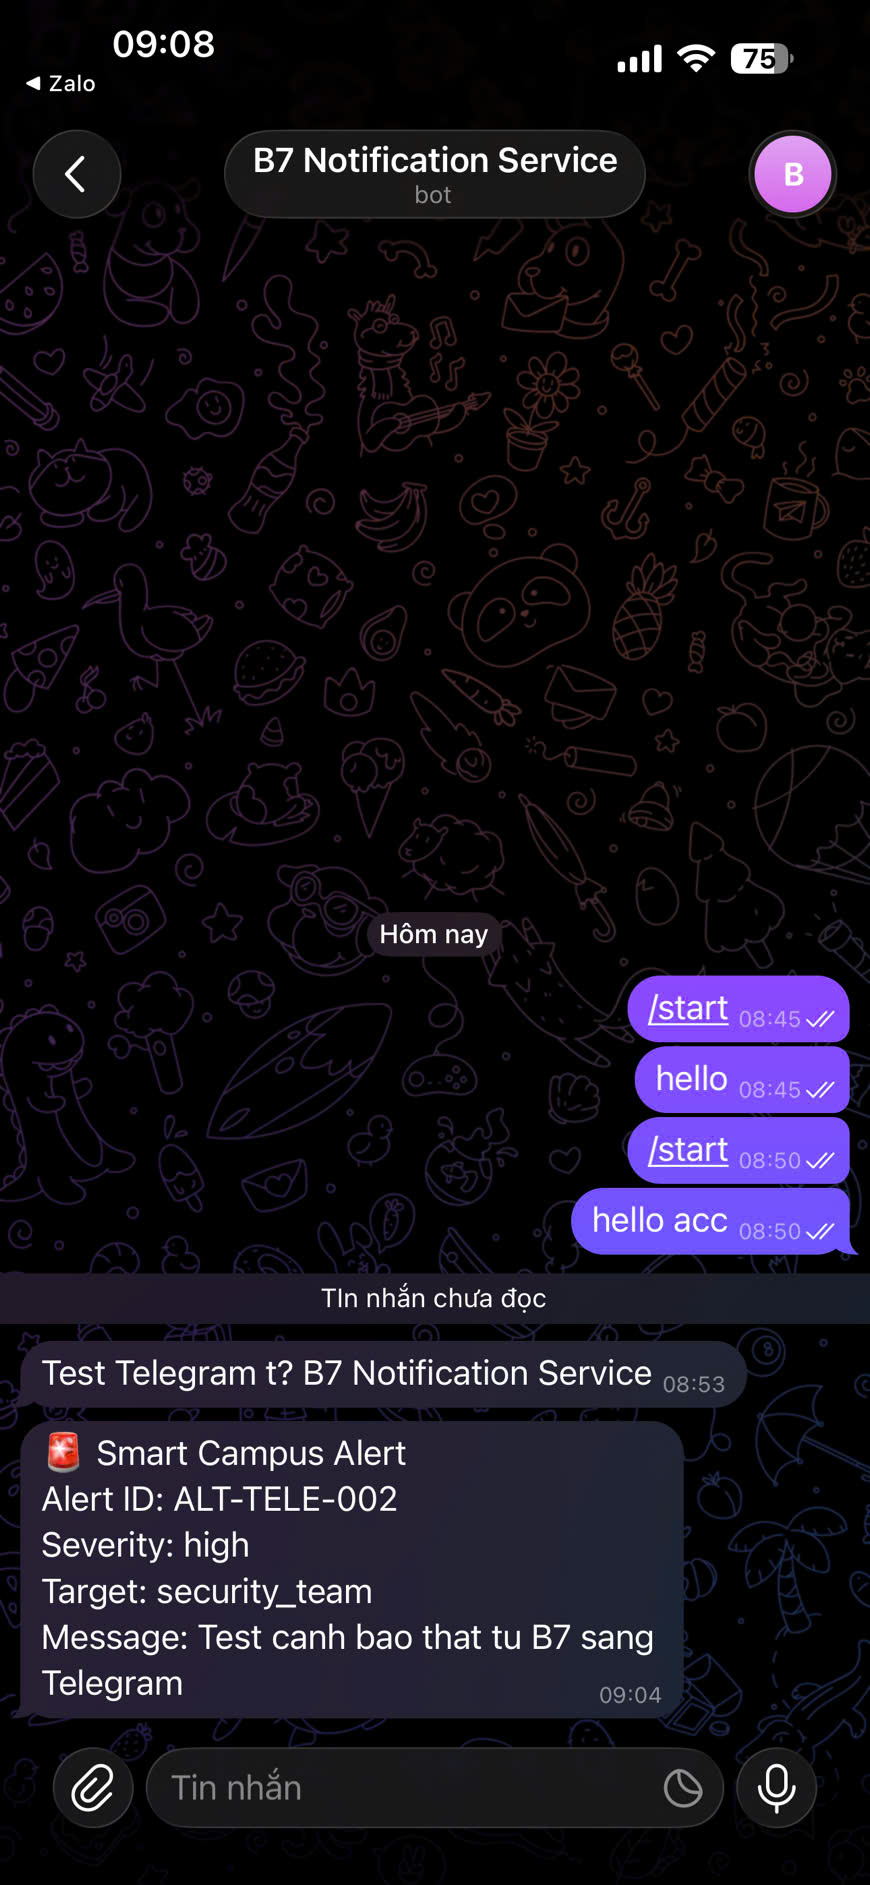
\includegraphics[width=0.45\textwidth]{images/telegram.png}
\caption{Thông báo được gửi thành công tới Telegram thông qua Notification Service}
\label{fig:telegram}
\end{figure}

\begin{figure}[H]
\centering
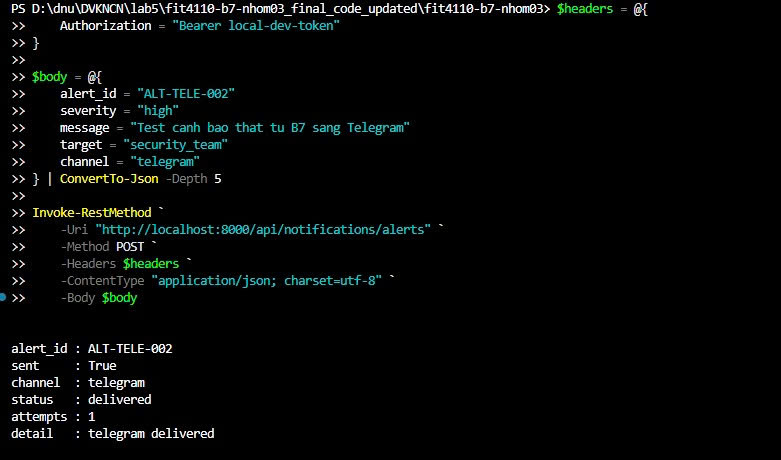
\includegraphics[width=\textwidth]{images/post-alert.png}
\caption{Kiểm thử API POST /api/notifications/alerts bằng PowerShell}
\label{fig:post}
\end{figure}

\begin{figure}[H]
\centering
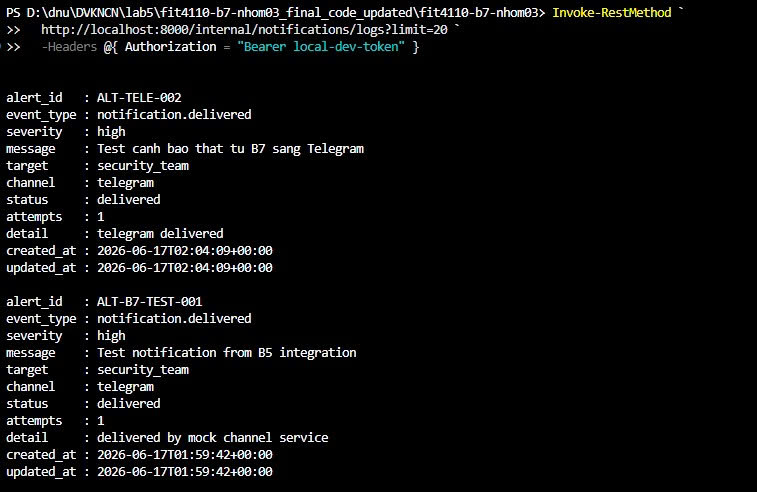
\includegraphics[width=\textwidth]{images/logs-api.png}
\caption{Kết quả truy xuất lịch sử thông báo thông qua Logs API}
\label{fig:logs}
\end{figure}

\begin{figure}[H]
\centering
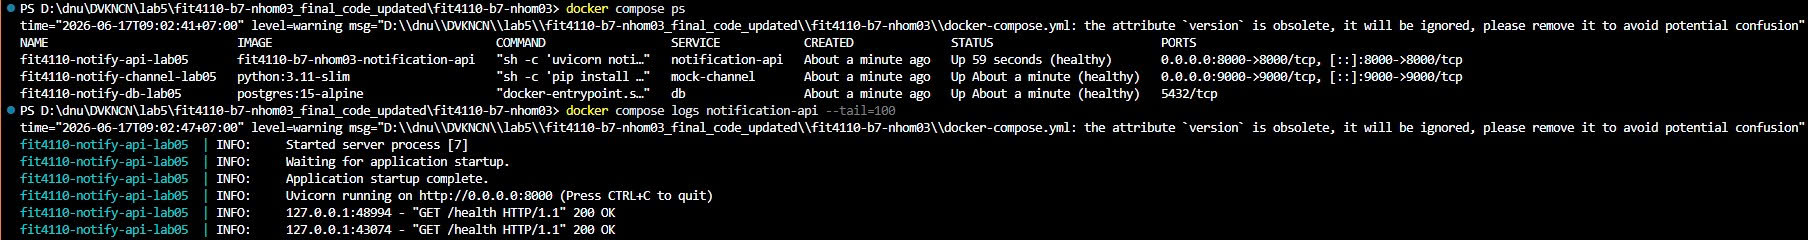
\includegraphics[width=\textwidth]{images/docker-compose.png}
\caption{Notification Service triển khai thành công bằng Docker Compose}
\label{fig:docker}
\end{figure}

%=========================================================
\section*{PHỤ LỤC B. CẤU TRÚC DỰ ÁN}

Cấu trúc thư mục chính của Notification Service được tổ chức như sau:

\begin{verbatim}

FIT4110-B7-NHOM03/
│
├── contracts/
│   └── team-notify.openapi.yaml
│
├── postman/
│   ├── collections/
│   └── environments/
│
├── reports/
│
├── src/
│   ├── mock_channel/
│   │   └── main.py
│   │
│   └── notify_app/
│       ├── __init__.py
│       └── main.py
│
├── .env
├── .env.example
├── docker-compose.yml
├── Dockerfile
├── lab05-check.yml
├── Makefile
├── README.md
├── requirements.txt
└── RUN_COMPOSE.md

\end{verbatim}

Trong đó:

\begin{itemize}

\item \textbf{contracts}: Chứa tài liệu OpenAPI Specification phục vụ tích hợp giữa các nhóm.

\item \textbf{postman}: Chứa Postman Collection và Environment phục vụ kiểm thử API.

\item \textbf{reports}: Chứa kết quả kiểm thử và báo cáo.

\item \textbf{src/mock\_channel}: Mock Channel mô phỏng việc gửi thông báo.

\item \textbf{src/notify\_app}: Thành phần chính của Notification Service.

\item \textbf{docker-compose.yml}: Triển khai toàn bộ hệ thống bằng Docker Compose.

\item \textbf{Dockerfile}: Đóng gói Notification Service thành Docker Image.

\item \textbf{requirements.txt}: Danh sách các thư viện Python.

\item \textbf{team-notify.openapi.yaml}: Đặc tả hợp đồng API của Notification Service.

\end{itemize}

%=========================================================
\section*{PHỤ LỤC C. CÁC API CHÍNH}

Notification Service cung cấp các REST API sau:

\begin{itemize}

\item GET /health

\item POST /api/notifications/alerts

\item GET /internal/notifications/logs

\item GET /internal/notifications/\{alert\_id\}/status

\item POST /internal/notifications/\{alert\_id\}/retry

\end{itemize}

Các API trên được sử dụng để tích hợp với Core Business Service (B6), Analytics Service (B5) và phục vụ quá trình kiểm thử hệ thống.

%=========================================================
\section*{PHỤ LỤC D. CÁC THÀNH PHẦN MÃ NGUỒN CHÍNH}

Các thành phần quan trọng của Notification Service gồm:

\begin{itemize}

\item \textbf{src/notify\_app/main.py}: Chứa toàn bộ logic xử lý của Notification Service, bao gồm xác thực Bearer Token, tiếp nhận Alert, gửi thông báo, Retry và Logs API.

\item \textbf{src/mock\_channel/main.py}: Mô phỏng Telegram Channel để phục vụ kiểm thử.

\item \textbf{docker-compose.yml}: Khởi tạo Notification API, PostgreSQL và Mock Channel.

\item \textbf{Dockerfile}: Đóng gói ứng dụng thành Docker Image.

\item \textbf{team-notify.openapi.yaml}: Đặc tả OpenAPI phục vụ tích hợp giữa các nhóm.

\item \textbf{Postman Collection}: Hỗ trợ kiểm thử các REST API của Notification Service.

\end{itemize}

%=========================================================
\section*{PHỤ LỤC E. TRIỂN KHAI HỆ THỐNG}

Notification Service được triển khai bằng Docker Compose với ba container:

\begin{itemize}

\item notification-api

\item db (PostgreSQL)

\item mock-channel

\end{itemize}

Các container được cấu hình hoạt động đồng thời nhằm đảm bảo Notification Service có thể xử lý yêu cầu, lưu trữ dữ liệu và mô phỏng quá trình gửi thông báo.

%=========================================================
\section*{PHỤ LỤC F. OPENAPI SPECIFICATION}

Notification Service sử dụng tài liệu OpenAPI Specification để mô tả các REST API phục vụ tích hợp với các nhóm khác trong hệ thống Smart Campus.

Tệp OpenAPI của hệ thống:

\begin{center}

\texttt{contracts/team-notify.openapi.yaml}

\end{center}

%=========================================================
```latex
\section*{PHỤ LỤC G. LIÊN KẾT MÃ NGUỒN}

Toàn bộ mã nguồn của Notification Service được quản lý bằng hệ thống Git và lưu trữ trên GitHub nhằm phục vụ quá trình phát triển, quản lý phiên bản và tích hợp giữa các thành viên trong nhóm.

\begin{itemize}

\item \textbf{Repository chính của dự án:}

\texttt{https://github.com/chuanvdn05/FIT4110-B7-NHOM03}

\item \textbf{OpenAPI Contract:}

\texttt{contracts/team-notify.openapi.yaml}

\item \textbf{Docker Compose:}

\texttt{docker-compose.yml}

\item \textbf{Dockerfile:}

\texttt{Dockerfile}

\item \textbf{Tài liệu hướng dẫn triển khai:}

\texttt{README.md}

\end{itemize}
```


%=========================================================
\section*{PHỤ LỤC H. KỊCH BẢN KIỂM THỬ}

Quy trình kiểm thử Notification Service được thực hiện theo các bước:

\begin{enumerate}

\item Khởi động hệ thống bằng Docker Compose.

\item Kiểm tra trạng thái Health Check thông qua endpoint GET /health.

\item Gửi Alert từ Core Business Service (B6).

\item Notification Service tiếp nhận, xác thực Bearer Token và xử lý yêu cầu.

\item Gửi thông báo tới Telegram.

\item Lưu lịch sử xử lý vào PostgreSQL.

\item Analytics Service (B5) truy xuất dữ liệu thông qua Logs API.

\end{enumerate}
```
